%==============================================================================
% tento soubor pouzijte jako zaklad
% this file should be used as a base for the thesis
% Autoři / Authors: 2008 Michal Bidlo, 2016 Jaroslav Dytrych
% Kontakt pro dotazy a připomínky: dytrych@fit.vutbr.cz
% Contact for questions and comments: dytrych@fit.vutbr.cz
%==============================================================================
% kodovani: UTF-8 (zmena prikazem iconv, recode nebo cstocs)
% encoding: UTF-8 (you can change it by command iconv, recode or cstocs)
%------------------------------------------------------------------------------
% zpracování / processing: make, make pdf, make clean
%==============================================================================
% Soubory, které je nutné upravit: / Files which have to be edited:
%   xkolcu00-Urceni-typu-a-smeru-zbrane-20-literatura-bibliography.bib - literatura / bibliography
%   xkolcu00-Urceni-typu-a-smeru-zbrane-01-kapitoly-chapters.tex - obsah práce / the thesis content
%   xkolcu00-Urceni-typu-a-smeru-zbrane-30-prilohy-appendices.tex - přílohy / appendices
%==============================================================================
\documentclass[slovak]{fitthesis}
%\documentclass[]{fitthesis} % bez zadání - pro začátek práce, aby nebyl problém s překladem
%\documentclass[english]{fitthesis} % without assignment - for the work start to avoid compilation problem
%\documentclass[zadani]{fitthesis} % odevzdani do wisu - odkazy jsou barevné
%\documentclass[english,zadani]{fitthesis} % for submission to the IS FIT - links are color
%\documentclass[zadani,print]{fitthesis} % pro tisk - odkazy jsou černé
%\documentclass[zadani,cprint]{fitthesis} % pro barevný tisk - odkazy jsou černé, znak VUT barevný
%\documentclass[english,zadani,print]{fitthesis} % for the color print - links are black
%\documentclass[english,zadani,cprint]{fitthesis} % for the print - links are black, logo is color
% * Je-li práce psaná v anglickém jazyce, je zapotřebí u třídy použít 
%   parametr english následovně:
%   If thesis is written in english, it is necessary to use 
%   parameter english as follows:
%      \documentclass[english]{fitthesis}
% * Je-li práce psaná ve slovenském jazyce, je zapotřebí u třídy použít 
%   parametr slovak následovně:
%   If the work is written in the Slovak language, it is necessary 
%   to use parameter slovak as follows:
%      \documentclass[slovak]{fitthesis}
% * Je-li práce psaná v anglickém jazyce se slovenským abstraktem apod., 
%   je zapotřebí u třídy použít parametry english a enslovak následovně:
%   If the work is written in English with the Slovak abstract, etc., 
%   it is necessary to use parameters english and enslovak as follows:
%      \documentclass[english,enslovak]{fitthesis}

% Základní balíčky jsou dole v souboru šablony fitthesis.cls
% Basic packages are at the bottom of template file fitthesis.cls
% zde můžeme vložit vlastní balíčky / you can place own packages here

% Kompilace po částech (rychlejší, ale v náhledu nemusí být vše aktuální)
% Compilation piecewise (faster, but not all parts in preview will be up-to-date)
% \usepackage{subfiles}

% Nastavení cesty k obrázkům
% Setting of a path to the pictures
%\graphicspath{{obrazky-figures/}{./obrazky-figures/}}
%\graphicspath{{obrazky-figures/}{../obrazky-figures/}}

\usepackage{graphicx}
\graphicspath{ {obrazky-figures/} }

%---rm---------------
\renewcommand{\rmdefault}{lmr}%zavede Latin Modern Roman jako rm / set Latin Modern Roman as rm
%---sf---------------
\renewcommand{\sfdefault}{qhv}%zavede TeX Gyre Heros jako sf
%---tt------------
\renewcommand{\ttdefault}{lmtt}% zavede Latin Modern tt jako tt

% vypne funkci šablony, která automaticky nahrazuje uvozovky,
% aby nebyly prováděny nevhodné náhrady v popisech API apod.
% disables function of the template which replaces quotation marks
% to avoid unnecessary replacements in the API descriptions etc.
\csdoublequotesoff

% =======================================================================
% balíček "hyperref" vytváří klikací odkazy v pdf, pokud tedy použijeme pdflatex
% problém je, že balíček hyperref musí být uveden jako poslední, takže nemůže
% být v šabloně
% "hyperref" package create clickable links in pdf if you are using pdflatex.
% Problem is that this package have to be introduced as the last one so it 
% can not be placed in the template file.
\ifWis
\ifx\pdfoutput\undefined % nejedeme pod pdflatexem / we are not using pdflatex
\else
  \usepackage{color}
  \usepackage[unicode,colorlinks,hyperindex,plainpages=false,pdftex]{hyperref}
  \definecolor{links}{rgb}{0.4,0.5,0}
  \definecolor{anchors}{rgb}{1,0,0}
  \def\AnchorColor{anchors}
  \def\LinkColor{links}
  \def\pdfBorderAttrs{/Border [0 0 0] }  % bez okrajů kolem odkazů / without margins around links
  \pdfcompresslevel=9
\fi
\else % pro tisk budou odkazy, na které se dá klikat, černé / for the print clickable links will be black
\ifx\pdfoutput\undefined % nejedeme pod pdflatexem / we are not using pdflatex
\else
  \usepackage{color}
  \usepackage[unicode,colorlinks,hyperindex,plainpages=false,pdftex,urlcolor=black,linkcolor=black,citecolor=black]{hyperref}
  \definecolor{links}{rgb}{0,0,0}
  \definecolor{anchors}{rgb}{0,0,0}
  \def\AnchorColor{anchors}
  \def\LinkColor{links}
  \def\pdfBorderAttrs{/Border [0 0 0] } % bez okrajů kolem odkazů / without margins around links
  \pdfcompresslevel=9
\fi
\fi
% Řešení problému, kdy klikací odkazy na obrázky vedou za obrázek
% This solves the problems with links which leads after the picture
\usepackage[all]{hypcap}

% Informace o práci/projektu / Information about the thesis
%---------------------------------------------------------------------------
\projectinfo{
  %Prace / Thesis
  project={BP},            %typ práce BP/SP/DP/DR  / thesis type (SP = term project)
  year={2018},             % rok odevzdání / year of submission
  date=\today,             % datum odevzdání / submission date
  %Nazev prace / thesis title
  title.cs={Určení typu a směru zbraně v obrazové scéně},  % název práce v češtině či slovenštině (dle zadání) / thesis title in czech language (according to assignment)
  title.en={Determination of Gun Type and Position in Image Scene}, % název práce v angličtině / thesis title in english
  %title.length={14.5cm}, % nastavení délky bloku s titulkem pro úpravu zalomení řádku (lze definovat zde nebo níže) / setting the length of a block with a thesis title for adjusting a line break (can be defined here or below)
  %Autor / Author
  author.name={Róbert},   % jméno autora / author name
  author.surname={Kolcún},   % příjmení autora / author surname 
  %author.title.p={Bc.}, % titul před jménem (nepovinné) / title before the name (optional)
  %author.title.a={Ph.D.}, % titul za jménem (nepovinné) / title after the name (optional)
  %Ustav / Department
  department={UITS}, % doplňte příslušnou zkratku dle ústavu na zadání: UPSY/UIFS/UITS/UPGM / fill in appropriate abbreviation of the department according to assignment: UPSY/UIFS/UITS/UPGM
  % Školitel / supervisor
  supervisor.name={Martin},   % jméno školitele / supervisor name 
  supervisor.surname={Drahanský},   % příjmení školitele / supervisor surname
  supervisor.title.p={Prof. Ing., Dipl.-Ing.},   %titul před jménem (nepovinné) / title before the name (optional)
  supervisor.title.a={Ph.D.},    %titul za jménem (nepovinné) / title after the name (optional)
  % Klíčová slova / keywords
  keywords.cs={Sem budou zapsána jednotlivá klíčová slova v českém (slovenském) jazyce, oddělená čárkami.}, % klíčová slova v českém či slovenském jazyce / keywords in czech or slovak language
  keywords.en={Sem budou zapsána jednotlivá klíčová slova v anglickém jazyce, oddělená čárkami.}, % klíčová slova v anglickém jazyce / keywords in english
  % Abstrakt / Abstract
  abstract.cs={Do tohoto odstavce bude zapsán výtah (abstrakt) práce v českém (slovenském) jazyce.}, % abstrakt v českém či slovenském jazyce / abstract in czech or slovak language
  abstract.en={Do tohoto odstavce bude zapsán výtah (abstrakt) práce v anglickém jazyce.}, % abstrakt v anglickém jazyce / abstract in english
  % Prohlášení (u anglicky psané práce anglicky, u slovensky psané práce slovensky) / Declaration (for thesis in english should be in english)
  declaration={Prohlašuji, že jsem tuto bakalářskou práci vypracoval samostatně pod vedením pana X...
Další informace mi poskytli...
Uvedl jsem všechny literární prameny a publikace, ze kterých jsem čerpal.},
  %declaration={Hereby I declare that this bachelor's thesis was prepared as an original author’s work under the supervision of Mr. X
% The supplementary information was provided by Mr. Y
% All the relevant information sources, which were used during preparation of this thesis, are properly cited and included in the list of references.},
  % Poděkování (nepovinné, nejlépe v jazyce práce) / Acknowledgement (optional, ideally in the language of the thesis)
  acknowledgment={V této sekci je možno uvést poděkování vedoucímu práce a těm, kteří poskytli odbornou pomoc
(externí zadavatel, konzultant, apod.).},
  %acknowledgment={Here it is possible to express thanks to the supervisor and to the people which provided professional help
%(external submitter, consultant, etc.).},
  % Rozšířený abstrakt (cca 3 normostrany) - lze definovat zde nebo níže / Extended abstract (approximately 3 standard pages) - can be defined here or below
  %extendedabstract={Do tohoto odstavce bude zapsán rozšířený výtah (abstrakt) práce v českém (slovenském) jazyce.},
  %faculty={FIT}, % FIT/FEKT/FSI/FA/FCH/FP/FAST/FAVU/USI/DEF
  faculty.cs={Fakulta informačních technologií}, % Fakulta v češtině - pro využití této položky výše zvolte fakultu DEF / Faculty in Czech - for use of this entry select DEF above
  faculty.en={Faculty of Information Technology}, % Fakulta v angličtině - pro využití této položky výše zvolte fakultu DEF / Faculty in English - for use of this entry select DEF above
  department.cs={Ústav matematiky}, % Ústav v češtině - pro využití této položky výše zvolte ústav DEF nebo jej zakomentujte / Department in Czech - for use of this entry select DEF above or comment it out
  department.en={Institute of Mathematics} % Ústav v angličtině - pro využití této položky výše zvolte ústav DEF nebo jej zakomentujte / Department in English - for use of this entry select DEF above or comment it out
}

% Rozšířený abstrakt (cca 3 normostrany) - lze definovat zde nebo výše / Extended abstract (approximately 3 standard pages) - can be defined here or above
%\extendedabstract{Do tohoto odstavce bude zapsán výtah (abstrakt) práce v českém (slovenském) jazyce.}

% nastavení délky bloku s titulkem pro úpravu zalomení řádku - lze definovat zde nebo výše / setting the length of a block with a thesis title for adjusting a line break - can be defined here or above
%\titlelength{14.5cm}


% řeší první/poslední řádek odstavce na předchozí/následující stránce
% solves first/last row of the paragraph on the previous/next page
\clubpenalty=10000
\widowpenalty=10000

\begin{document}
  % Vysazeni titulnich stran / Typesetting of the title pages
  % ----------------------------------------------
  \maketitle
  % Obsah
  % ----------------------------------------------
  \setlength{\parskip}{0pt}

  {\hypersetup{hidelinks}\tableofcontents}
  
  % Seznam obrazku a tabulek (pokud prace obsahuje velke mnozstvi obrazku, tak se to hodi)
  % List of figures and list of tables (if the thesis contains a lot of pictures, it is good)
  \ifczech
    \renewcommand\listfigurename{Seznam obrázků}
  \fi
  \ifslovak
    \renewcommand\listfigurename{Zoznam obrázkov}
  \fi
  % \listoffigures
  
  \ifczech
    \renewcommand\listtablename{Seznam tabulek}
  \fi
  \ifslovak
    \renewcommand\listtablename{Zoznam tabuliek}
  \fi
  % \listoftables 

  \ifODSAZ
    \setlength{\parskip}{0.5\bigskipamount}
  \else
    \setlength{\parskip}{0pt}
  \fi

  % vynechani stranky v oboustrannem rezimu
  % Skip the page in the two-sided mode
  \iftwoside
    \cleardoublepage
  \fi

  % Text prace / Thesis text
  % ----------------------------------------------
  \chapter{Úvod}

%\section{Úvod a motivácia}
Žvasty o tom koľko je útokov zbrani v ČR a pod...


% ------------ NEW CHAPTER ------------
\chapter{Technológie}

V tejto kapitole sa zoznámime so základnymi pojmami a princípmi, ktoré súvia s probletikou tejto práce a ktoré budú dalej využívané.
Kapitola vysvetľuje základne rozdelenia zbraní, princíp spracovania digitálneho obrazu a metódy jeho predspracovanie.
Ďalej sú tu vysvetlené rôzne spôsoby pre klasifikáciu týchto obrazových dát.

% http://scikit-learn.org/stable/tutorial/machine\_learning\_map/index.html
% 16008.pdf - Klasifikacne algoritmy - str.10+
% imagenet-classification-with-deep-convolutional-neural-networks.pdf - Introduction str.1+
% Rozpoznávání-termosnímků-obličeju.pdf
% 9614.pdf

\section{Zbrane}
Obvýklá definícia hovorí, že zbraň je nástroj, predmet, či dokonca celé zariadenie,
ktoré je prispôsobené k vyvolaniu ranivého účinku na živý organizmus alebo k ničeniu objektu\cite{book:StrelneZbrane}.
Za prvé zbrane môžeme považovať kopije ktoré používali luďia pri love zvierat asi pred 400,000 rokmi\cite{prop:SpearHistory}.

Vo všeobecnosti môžeme zbrane rozdeliť podľa množstvá krytérií, napr. podľa zdroja energie použitej k vypudeniu projektilu zo zbrane,
podľa konštrukcie a režimu streľby, ďalej z hľadiska postupu pri nabíjaní alebo podľa veku zbrane na nové - slúžiace svojmu účelu a historické - ktoré sú uź nespôsobilé k pôvodnemu účelu.
My sa zameriame na 2 základne rozdelenia a to poďla toho ako zbrane pôsobia na živú sílu[cz. živou sílu], delíme na\cite{book:StrelneZbrane}:
\begin{enumerate}
	\item[$\bullet$] \textbf{Strelné} - rozrušujú vzdialený cieľ, živý alebo neživý, prodstredníctvom depadovej energie strely vypudenej zo zbrane.
	\item[$\bullet$] \textbf{Chladné} - účinkujú bodom alebo sekom naostrenej čepele, ktorá je vsadená do rukoväťe lebo je nasadená na tyč alebo porísko.
    \item[$\bullet$] \textbf{Úderné} - pôsobia na živý objekt tupým úderom s vojej časti, tkorá býva spojená s vhodnou rukoväťou.
\end{enumerate}
a podľa ovládateľnosti a možnosti prenášania ich delíme na\cite{book:StrelneZbrane}:
\begin{enumerate}
	\item[$\bullet$] \textbf{Ručné} strelné zbrane môže prenášať a ovládať jediná osoba. Sú ovládané buď jednou rukou - krátke zbrane - alebo oboma rukami - dlhé zbrane.
	\item[$\bullet$] \textbf{Lafetované} zbrane musia byť vzhľadom ku svojej hmotnosti a rozmerom umiestnené na zvláštnom podstavci - \textit{lafete}. Takúto zbraň takisto väčsinou obsluhuje viac ľudí.
\end{enumerate}
V tejto práci sa zameramé hlavne na strelné, ručné zbrane.

\section{Spracovanie obrazu}
Pre popis obrázkov a ostatných signálov sú často používané matematické modely.
Kde signál je funkcia závislá na nejakých premenných s fyzikálnym významom, môže byť 1-dimenzionálna (napr. závisla na čase),
2-dimenzionálna (napr. obrázok závislý na 2 koordinátoch v ploche), 3-dimenzionálna (napr. popis pozície objektu v priestore), alebo aj viac-dimenzionálna\cite{book:ImageProcessing}.

    Každý obraz môže byť definovaný ako spojitá funkcia s dvomi neznámymi $$f(x,y)$$ kde $x$ a $y$ sú súradnice v ploche.
Tento spojitý obraz je digitalizovaný na tzv. vzorkovacích miestach.
Tieto vzorkovacie miesta sú usporiadané v ploche, ich geometrický vzťah sa nazýva mriežka.
Digitálny obraz je potom dátova štruktúra, ktorá je bežne reprezentovaná ako matica.
Jeden bod v mriežke reprezentuje jeden element 2-dimenzionálneho obraze nazývany pixel, v 3-dimenzionálnom obraze sá tento element nazýva voxel\cite{book:ImageProcessing}.
Pri viac-dimenzionálnych digitálnych obrazoch sa pri spracovaní obrazu používa vektor hodnôt(napr. RGB hodnoty obrazového bodu).

Oblasť spracovania digitálneho obrazu je v dnešnej dobe veľmi široká a nachádza uplatnenie vo viacerých oboroch.
Môže sa využívať pri automatickej vizuálnej inšpekcií produktou, pre zaistenie vyššej produktivity a kvality výrobku v továrňach.
Ďalej pri spracovaní snímkou z lietadiel alebo satelitou pre získanie dát o prírodnych zdrojoch, ako napr. v poľnohospodárstve alebo lesníctve.
Širokú aplikáciu má v medicíne pri obrázkoch získavaných pomocou röngenových zariadení, CT a magnetickej rezonancie\cite{book:ImageProcessingApplication}.
A v súčastnosti v automobilovom priemysle pri rozvýjajúcej sa oblati autonómneho riadenia automobilov.

\section{Klasifikácia}

\# TODO - dopisať čo je to Klasifikácia

\subsection{K-Nearest-Neighbor}
\textit{k}-Nearest Neighbor je algoritmus ktorý sa učí pod dozorom [eng. supervised learning algorithm] často používaný pri rozpoznávaní vzorov v klasifikácií,
avšak je možné ho použiť aj pre odhad a predikciu\cite{book:DataMining}.
Algoritmus je pamäťovo náročný [eng. memory-based] a nepotrebuje žiaden model.
Pre jeho fungovanie nie je potrebný žiaden explicitný postup trénovania, okrem zberu vektorov príznakov s označeniami tried do ktorých patria.

Klasifikácia dát prebieha v 2 krokoch: nájdenie \textit{k} najbližších susedov spomedzi trénovaných dát a
vykonanie "väčšinové hlasovanie" medzi nájdenými susedmi pre priradenie najčastejšie sa vykytovaného označenia triedy.

Nech $\{ (x_i, y_i), i = 1, 2, \dots, n \}$ je množína trénovacích dát, kde $x_i$ je vektor príznakov a $y_i$ je názov triedy do ktorej patrí vektor $x_i$.
Predpokladáme že každé $x_i$ je v nejakom multidimenzionálnom priestore príznakov s metrikov $P$ a $y_i \in \{ 1, 2, \dots, l \}$, kde $l$ je číslo odpovedajúcej triedy.
Cieľom je priradiť neoznačeny vektor $x$ do zodpovedajucej triedy z množiny $\{ 1, 2, \dots, l \}$.

Najjednoduchšia verzia algoritmu \textit{k}-NN je 1-NN, kde vektor $x$ je priradený najbližsiemu susedovy.
To znamená že ak $x_j$, kde $j \in \{ 1, 2, \dots, n \}$, je najbližšií k $x$ vo forme vzdialenosti $P$ \cite{prop:KnnClassification}:
\begin{equation}
    \label{eq:kNNMetric}
    x_j = arg \; min_{\{x_i, 1 \leq i \leq n\}} P(x, x_i)
\end{equation}
tak označenie triedy pre vektor $x$ je číslo $y_i$.

Pre formu algoritmu \textit{k}-NN, kde $k > 1$ je postup podobný, ale priradenie označenia triedy pre $x$ je na základe najčastejšie sa vyskutovaného označenia triedy
spomedzi \textit{k} najbližších susedov z trénovacých bodov $x_i$, kde $k$ je užívateľom definovaná konštanta \cite{prop:KnnClassification}.

Najbežnejší výpočet pre vzdielenosť bodov je pomocou Euklidovskej vzdielenosti.
Táto vzdielnosť je medzi dvoma $J$-dimenzionálnymi vektormi $a$ a $b$ vyjadrená ako \cite{prop:KnnClassification}:
\begin{equation}
    \label{eq:euclidMetric}
    d_{a,b} = \sqrt{\sum_{j=1}^{J}{(a_j - b_j)^2}}
\end{equation}

Na obrázku \ref{pic:kNN} je zobrazený rozdiel medzi 1-NN a 5-NN algoritmom pre klasifikáciou,
    použitím 2-dimenzionálnych bodov a 3 tried dát (červená, modrá, zelená).
Farebné regióny vyznačujú rozhodovacie hranice klasifikátora, ktorý využíva Euklidovskú vzdielnosť.
Biele oblasti ukazujú body, ktoré sú nejednoznačne klasifikované (to znamená, že hodnotenie triedy je viazané aspoň na dve triedy).
V ukážke je vidno že v prípade 1-NN klasifikátora, niektré body vytvárajú "malé ostrovy"
    (napr. zelený bod v strede mraku medzi modrými bodmi), zatiaľ čo 5-NN klasifikátor vyhladzuje tieto nezrovnalosti,
    a pravdepodobne vedie k lepšiemu zovšeobecneniu nad testovacími údajmi.

\begin{figure}[H]
	\centering
	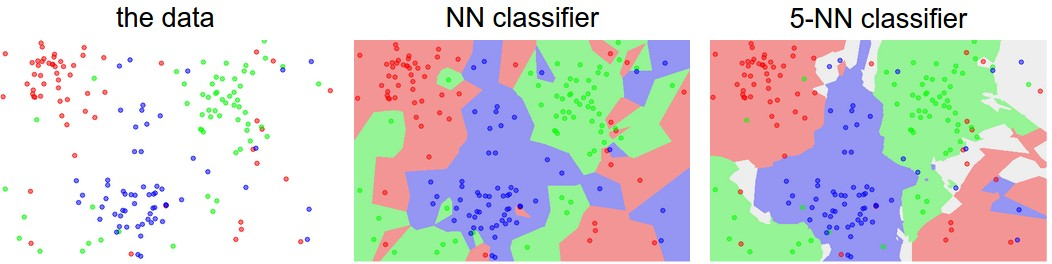
\includegraphics[width=1\textwidth]{knn}
	\caption{Porovnanie k-NN klasifikátorov}
	\label{pic:kNN}
\end{figure}

\# TODO odkaz na obrazok

\subsection{Support Vector Machines}

\subsection{Stochastic Gradient Descent}

\subsection{Neural Network}
- 17150\_FULLTEXT.pdf - Background str.25, Deep learning str.30

- DiplomovaPraca.pdf - HLBOKÉ UČENIE A NEURÓNOVÉ SIETE str.20

- DP\_MajtánMartin.pdf - 1 NEURÓNOVÉ\ SIETE str.10

- FIT\_neuronky.pdf - Kap 3 Neuronové siete str.21

O čom je všeobecne Maching Learning
[Useful-things-about-machine-learning]

Machine Learning sa pouziva v širokej škále oblasti npr .....
My sme sa rozhodli použit ho na detekovanie typu zbrane a náklonu zbrane v obrazovej scéne.


%\subsection{Decision Trees}
%Asi NIE
%http://scikit-learn.org/stable/modules/tree.html


\section{Predspracovanie obrazu}
http://scikit-image.org/docs/dev/auto\_examples/

\subsection{Hogova transformacia}
- F3-DP-2016-Erlebach-Jonas-Automaticka detekce pupily v obraze.pdf

\subsection{Detekcia hran}

- Sobelov filter - podľa knižky patri medzi najpopulárnejšie hranové filter.
Urobiť z neho magnitúdu obrazu potom.

% ------------ NEW CHAPTER ------------
\chapter{Návrh riešenia}

- Exploiting-the-complementary-strengths-of-multi-layer-CNN-image-retrieval.pdf,
preco pouzivat CNN na tento problem

\section{Keras}
- 17150\_FULLTEXT.pdf - Tensorflow and Keras str.26

- Navrhovana technologia pre ucenie

\section{scikit-learn}
- Kratky popis

\section{Databáza zbraní}
- ....

\section{Klasifikácia typu zbrane}

\section{Určenie natočenia zbrane}


% ------------ NEW CHAPTER ------------
\pagebreak
\chapter{Implementácia}

\section{Dataset}

  
  % Kompilace po částech (viz výše, nutno odkomentovat)
  % Compilation piecewise (see above, it is necessary to uncomment it)
  %\subfile{projekt-01-uvod-introduction}
  % ...
  %\subfile{chapters/projekt-05-conclusion}


  % Pouzita literatura / Bibliography
  % ----------------------------------------------
\ifslovak
  \makeatletter
  \def\@openbib@code{\addcontentsline{toc}{chapter}{Literatúra}}
  \makeatother
  \bibliographystyle{bib-styles/czechiso}
\else
  \ifczech
    \makeatletter
    \def\@openbib@code{\addcontentsline{toc}{chapter}{Literatura}}
    \makeatother
    \bibliographystyle{bib-styles/czechiso}
  \else 
    \makeatletter
    \def\@openbib@code{\addcontentsline{toc}{chapter}{Bibliography}}
    \makeatother
    \bibliographystyle{bib-styles/englishiso}
  %  \bibliographystyle{alpha}
  \fi
\fi
  \begin{flushleft}
  \bibliography{xkolcu00-Urceni-typu-a-smeru-zbrane-20-literatura-bibliography}
  \end{flushleft}

  % vynechani stranky v oboustrannem rezimu
  % Skip the page in the two-sided mode
  \iftwoside
    \cleardoublepage
  \fi

  % Prilohy / Appendices
  % ---------------------------------------------
  \appendix
\ifczech
  \renewcommand{\appendixpagename}{Přílohy}
  \renewcommand{\appendixtocname}{Přílohy}
  \renewcommand{\appendixname}{Příloha}
\fi
\ifslovak
  \renewcommand{\appendixpagename}{Prílohy}
  \renewcommand{\appendixtocname}{Prílohy}
  \renewcommand{\appendixname}{Príloha}
\fi
%  \appendixpage

% vynechani stranky v oboustrannem rezimu
% Skip the page in the two-sided mode
%\iftwoside
%  \cleardoublepage
%\fi
  
\ifslovak
%  \section*{Zoznam príloh}
%  \addcontentsline{toc}{section}{Zoznam príloh}
\else
  \ifczech
%    \section*{Seznam příloh}
%    \addcontentsline{toc}{section}{Seznam příloh}
  \else
%    \section*{List of Appendices}
%    \addcontentsline{toc}{section}{List of Appendices}
  \fi
\fi
  \startcontents[chapters]
  \setlength{\parskip}{0pt}
  % seznam příloh / list of appendices
  % \printcontents[chapters]{l}{0}{\setcounter{tocdepth}{2}}
  
  \ifODSAZ
    \setlength{\parskip}{0.5\bigskipamount}
  \else
    \setlength{\parskip}{0pt}
  \fi
  
  % vynechani stranky v oboustrannem rezimu
  \iftwoside
    \cleardoublepage
  \fi
  
  % Přílohy / Appendices
  % Tento soubor nahraďte vlastním souborem s přílohami (nadpisy níže jsou pouze pro příklad)
% This file should be replaced with your file with an appendices (headings below are examples only)

% Umístění obsahu paměťového média do příloh je vhodné konzultovat s vedoucím
% Placing of table of contents of the memory media here should be consulted with a supervisor
%\chapter{Obsah přiloženého paměťového média}

%\chapter{Manuál}

%\chapter{Konfigurační soubor} % Configuration file

%\chapter{RelaxNG Schéma konfiguračního souboru} % Scheme of RelaxNG configuration file

%\chapter{Plakát} % poster

  
  % Kompilace po částech (viz výše, nutno odkomentovat)
  % Compilation piecewise (see above, it is necessary to uncomment it)
  %\subfile{xkolcu00-Urceni-typu-a-smeru-zbrane-30-prilohy-appendices}
  
\end{document}
